\label{sec:kuramoto}
\subsection{Definition}
The problem of having a naive viewpoint on the subject of synchronization is that one may believe that every different coupling situation would require its own treatment. This may stem from the fact that one may be focusing too much on the differences rather then the similarities which are found in all synchronous systems. One such attempt to define these similarities in a mathematical form was proposed by Kuramoto in 1975.
\[
\dot{\theta_i} = \omega_i + \sum_{j = 0}^{N}{A_{i, j}\sin({\theta_j - \theta_i}}
)\]
where:
\begin{itemize}
	\item[${\theta_i} = $] The phase of the $i\textsuperscript{th}$ oscillator
	\item[$\omega_i = $] The natural frequency of the $i\textsuperscript{th}$ oscillator
	\item[$A_{i, j} = $] The adjacency matrix of the system
\end{itemize}
~\\
Each oscillator has its own natural frequency which is held when kept in isolation but when coupled with other oscillators, it changes. This change is periodic and is thus represented by the periodic $\sin$ function.

\ednote{Alee: Write about the system: Describe the equation in general and what each constant means. No graphs here yet, just the basic explanation. }
\ednote{Alee: Write about the simulation we have written, i.e. we used Numpy, we have a script that can handle arbritrary parameters and make a simple **positive coefficient** system where you can explain the connection. }
\ednote{Alee[potentially saturday]: Write about system stability (i. e. switch to a constant frame of reference, find fix points and take the Jacobian)}


\subsection{Adjacency Matrix and the Network Topology }
Now we move on to define the mathematical tools being used in this project. The Adjacency matrix is a square matrix that is using to represent a finite graph. The elements of the matrix indicate whether pairs of verticies are adjacent or not, ie if they are adjacent they get assigned a value of -1 else 0. This information can be directly retrieved from the topology network graph as follows-:

\begin{figure}[h!]
\centering
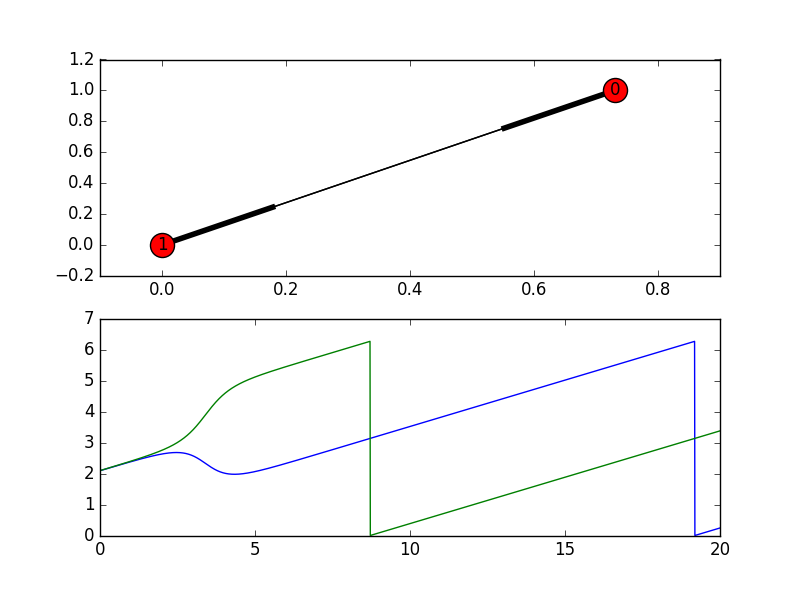
\includegraphics[width=\linewidth]{imgs/examplefigure}
\caption{}
\end{figure}

As we can see, on the top is the topological network containing the vertices of the system and below lies the coupling graphs of the system over time. Over here, we can see that the couples are trying to stay as far away as possible so after the initial unrest there is always a phase difference of 2$\pi$. \ednote{JUST show the graph and the adjacency matrix here. This is ONLY the introduction. }
